\documentclass[a4paper]{book}
\usepackage{a4wide}
\usepackage{makeidx}
\usepackage{fancyhdr}
\usepackage{graphicx}
\usepackage{multicol}
\usepackage{float}
\usepackage{textcomp}
\usepackage{alltt}
\usepackage{times}
\usepackage{ifpdf}
\ifpdf
\usepackage[pdftex,
            pagebackref=true,
            colorlinks=true,
            linkcolor=blue,
            unicode
           ]{hyperref}
\else
\usepackage[ps2pdf,
            pagebackref=true,
            colorlinks=true,
            linkcolor=blue,
            unicode
           ]{hyperref}
\usepackage{pspicture}
\fi
\usepackage[utf8]{inputenc}
\usepackage{doxygen}
\makeindex
\setcounter{tocdepth}{3}
\renewcommand{\footrulewidth}{0.4pt}
\begin{document}
\begin{titlepage}
\vspace*{7cm}
\begin{center}
{\Large Monde des cubes }\\
\vspace*{1cm}
{\large Generated by Doxygen 1.5.7.1}\\
\vspace*{0.5cm}
{\small Tue Mar 31 13:22:30 2009}\\
\end{center}
\end{titlepage}
\clearemptydoublepage
\pagenumbering{roman}
\tableofcontents
\clearemptydoublepage
\pagenumbering{arabic}
\chapter{Class Index}
\section{Class List}
Here are the classes, structs, unions and interfaces with brief descriptions:\begin{CompactList}
\item\contentsline{section}{\hyperlink{classEcoAgent}{EcoAgent} (Classe abstraite appelee par les classes Cube et Table )}{\pageref{classEcoAgent}}{}
\item\contentsline{section}{\hyperlink{classPlateformeEcoResolution}{PlateformeEcoResolution} (Classe representant une plateforme d'eco-resolution abstraite )}{\pageref{classPlateformeEcoResolution}}{}
\item\contentsline{section}{\hyperlink{classSingleton}{Singleton$<$ T $>$} (Template de classe permettant de rendre une classe instanciable une seule fois )}{\pageref{classSingleton}}{}
\end{CompactList}

\chapter{File Index}
\section{File List}
Here is a list of all documented files with brief descriptions:\begin{CompactList}
\item\contentsline{section}{trunk/include/\hyperlink{cube_8hpp}{cube.hpp} (Implementation du module cube qui est un derive d'un \hyperlink{classEcoAgent}{EcoAgent} )}{\pageref{cube_8hpp}}{}
\item\contentsline{section}{trunk/include/\hyperlink{ecoAgent_8hpp}{ecoAgent.hpp} (Mise en place de la classe abstraite \hyperlink{classEcoAgent}{EcoAgent} )}{\pageref{ecoAgent_8hpp}}{}
\item\contentsline{section}{trunk/include/\hyperlink{ecoAgentID_8hpp}{ecoAgentID.hpp} (Implementation de la classe \hyperlink{classEcoAgentID}{EcoAgentID} )}{\pageref{ecoAgentID_8hpp}}{}
\item\contentsline{section}{trunk/include/\hyperlink{etat_8hpp}{etat.hpp} (Enumeration des etats possibles des eco-agents )}{\pageref{etat_8hpp}}{}
\item\contentsline{section}{trunk/include/\hyperlink{plateformeEcoResolution_8hpp}{plateformeEcoResolution.hpp} (Plateforme abstraite d'eco-resolution )}{\pageref{plateformeEcoResolution_8hpp}}{}
\item\contentsline{section}{trunk/include/\hyperlink{plateformeMondeDesCubes_8hpp}{plateformeMondeDesCubes.hpp} (Plateforme d'eco-resolution appliquee au monde des cubes )}{\pageref{plateformeMondeDesCubes_8hpp}}{}
\item\contentsline{section}{trunk/include/\hyperlink{regle_8hpp}{regle.hpp} (Squelette d'une regle pour une plateforme d'eco-resolution )}{\pageref{regle_8hpp}}{}
\item\contentsline{section}{trunk/include/\hyperlink{singleton_8hpp}{singleton.hpp} (Implementation du design pattern singleton )}{\pageref{singleton_8hpp}}{}
\item\contentsline{section}{trunk/include/\hyperlink{table_8hpp}{table.hpp} (Implementation du module table qui est un derive d'un \hyperlink{classEcoAgent}{EcoAgent} )}{\pageref{table_8hpp}}{}
\end{CompactList}

\chapter{Class Documentation}
\hypertarget{classEcoAgent}{
\section{EcoAgent Class Reference}
\label{classEcoAgent}\index{EcoAgent@{EcoAgent}}
}
Classe abstraite appelee par les classes Cube et Table.  


{\tt \#include $<$ecoAgent.hpp$>$}



\subsection{Detailed Description}
Classe abstraite appelee par les classes Cube et Table. 

The documentation for this class was generated from the following file:\begin{CompactItemize}
\item 
include/\hyperlink{ecoAgent_8hpp}{ecoAgent.hpp}\end{CompactItemize}

\hypertarget{classPlateformeEcoResolution}{
\section{PlateformeEcoResolution Class Reference}
\label{classPlateformeEcoResolution}\index{PlateformeEcoResolution@{PlateformeEcoResolution}}
}
classe representant une plateforme d'eco-resolution abstraite  


{\tt \#include $<$plateformeEcoResolution.hpp$>$}

Inherited by \hyperlink{classPlateformeMondeDesCubes}{PlateformeMondeDesCubes}.

\subsection*{Public Member Functions}
\begin{CompactItemize}
\item 
\hyperlink{classPlateformeEcoResolution_6e03cc2c6a51bc4a47d2d226e41d13e9}{PlateformeEcoResolution} ()
\begin{CompactList}\small\item\em Constructeur. \item\end{CompactList}\item 
virtual \hyperlink{classPlateformeEcoResolution_356b4862f53c4be870304e5186601b5a}{$\sim$PlateformeEcoResolution} ()
\begin{CompactList}\small\item\em Destructeur. \item\end{CompactList}\item 
\hyperlink{classEcoAgent}{EcoAgent} $\ast$ \hyperlink{classPlateformeEcoResolution_acd4e2899f178261ddd0fde086932e84}{getEcoAgent} (const \hyperlink{classEcoAgentID}{EcoAgentID} \&id) const 
\begin{CompactList}\small\item\em Obtention d'un \hyperlink{classEcoAgent}{EcoAgent}. \item\end{CompactList}\item 
virtual void \hyperlink{classPlateformeEcoResolution_6fdb4c8ecc62252da4326d9763d4f28d}{addEcoAgent} (\hyperlink{classEcoAgent}{EcoAgent} \&ea)
\begin{CompactList}\small\item\em Ajout d'un \hyperlink{classEcoAgent}{EcoAgent}. \item\end{CompactList}\item 
void \hyperlink{classPlateformeEcoResolution_c2978a0e31b186415ca156a19ac8a1dc}{addRegle} (\hyperlink{classRegle}{Regle} \&r)
\begin{CompactList}\small\item\em Ajout d'une nouvelle regle. \item\end{CompactList}\item 
list$<$ \hyperlink{classRegle}{Regle} $\ast$ $>$ \hyperlink{classPlateformeEcoResolution_81dad57670e80ac2d29d02918b610636}{getRegles} ()
\begin{CompactList}\small\item\em Obtention de la liste des regles. \item\end{CompactList}\item 
bool \hyperlink{classPlateformeEcoResolution_0d35ee702a0b255f0da91aa382089865}{verifierCoherence} () const 
\begin{CompactList}\small\item\em Verification du respect des regles apres l'initialisation de la plateforme. \item\end{CompactList}\item 
bool \hyperlink{classPlateformeEcoResolution_673b4d17360ab1ff1e7c7f28a1b2e35e}{sontSatisfaits} () const 
\begin{CompactList}\small\item\em Methode qui verifie si tous les EcoAgents sont satisfaits i.e. si la resolution est terminee. \item\end{CompactList}\item 
\hyperlink{classEcoAgentID}{EcoAgentID} $\ast$ \hyperlink{classPlateformeEcoResolution_a33074c437f57bf9f409502de82b2f58}{getEcoAgentAuDessus} (const \hyperlink{classEcoAgentID}{EcoAgentID} \&id) const 
\begin{CompactList}\small\item\em Methode qui retourne l'EcoAgentID de l'EcoAgent au dessus. \item\end{CompactList}\item 
int \hyperlink{classPlateformeEcoResolution_bccb426d9f1113e66b652bb63e7fafcd}{nombreEcoAgentAuDessus} (const \hyperlink{classEcoAgentID}{EcoAgentID} \&id) const 
\begin{CompactList}\small\item\em Methode qui retourne le nombre d'EcoAgent au dessus de l'EcoAgent avec l'id specifie. \item\end{CompactList}\item 
list$<$ \hyperlink{classEcoAgentID}{EcoAgentID} $\ast$ $>$ \hyperlink{classPlateformeEcoResolution_eccbbf85153147e551b9b6fa65f554e2}{getEcoAgents} (const \hyperlink{etat_8hpp_767b7a63d7677f92d697621b4166af1b}{Etat} e) const 
\begin{CompactList}\small\item\em Methode qui retourne les \hyperlink{classEcoAgentID}{EcoAgentID} des \hyperlink{classEcoAgent}{EcoAgent} possedant l'etat specifie. \item\end{CompactList}\item 
map$<$ \hyperlink{classEcoAgentID}{EcoAgentID}, \hyperlink{classEcoAgent}{EcoAgent} \&, \hyperlink{structcompareEcoAgentID}{compareEcoAgentID} $>$ \hyperlink{classPlateformeEcoResolution_c3c3307a04fbe2d33c753c2b0eef79af}{getEcoAgents} () const 
\begin{CompactList}\small\item\em Methode qui retourne tous les eco-agents. \item\end{CompactList}\item 
virtual void \hyperlink{classPlateformeEcoResolution_57d87139f09ca51cd6a4fa7cd2e83351}{initialiser} ()=0
\begin{CompactList}\small\item\em Initialisation de la resolution. \item\end{CompactList}\item 
virtual void \hyperlink{classPlateformeEcoResolution_17f587580cd8aee537551bc0ddd82bef}{resoudre} ()=0
\begin{CompactList}\small\item\em Resolution du probleme par eco-resolution. \item\end{CompactList}\end{CompactItemize}
\subsection*{Protected Attributes}
\begin{CompactItemize}
\item 
map$<$ \hyperlink{classEcoAgentID}{EcoAgentID}, \hyperlink{classEcoAgent}{EcoAgent} \&, \hyperlink{structcompareEcoAgentID}{compareEcoAgentID} $>$ \hyperlink{classPlateformeEcoResolution_02de97d0d9dac3719ceaadfb255492a3}{ecoagents}
\item 
list$<$ \hyperlink{classRegle}{Regle} $\ast$ $>$ \hyperlink{classPlateformeEcoResolution_4f7dc37edf042a189073f15771604e35}{regles}
\end{CompactItemize}


\subsection{Detailed Description}
classe representant une plateforme d'eco-resolution abstraite 

La classe gere les fonctionnalites basiques d'une plateforme d'eco-resolution. Elle permet l'ajout d'EcoAgent et les references grace a leur identifiant \hyperlink{classEcoAgentID}{EcoAgentID}. Elle integre un ensemble de fonctionnalites \char`\"{}basiques\char`\"{} qui permettent par exemple d'obtenir un \hyperlink{classEcoAgent}{EcoAgent} reference a partir de son ID, d'ajouter des regles et de les verifier. Bien evidemment, la plateforme permet de lancer la resolution en elle-meme. 

\subsection{Constructor \& Destructor Documentation}
\hypertarget{classPlateformeEcoResolution_6e03cc2c6a51bc4a47d2d226e41d13e9}{
\index{PlateformeEcoResolution@{PlateformeEcoResolution}!PlateformeEcoResolution@{PlateformeEcoResolution}}
\index{PlateformeEcoResolution@{PlateformeEcoResolution}!PlateformeEcoResolution@{PlateformeEcoResolution}}
\subsubsection[{PlateformeEcoResolution}]{\setlength{\rightskip}{0pt plus 5cm}PlateformeEcoResolution::PlateformeEcoResolution ()}}
\label{classPlateformeEcoResolution_6e03cc2c6a51bc4a47d2d226e41d13e9}


Constructeur. 

Constructeur de la classe abstraite \hyperlink{classPlateformeEcoResolution}{PlateformeEcoResolution} \hypertarget{classPlateformeEcoResolution_356b4862f53c4be870304e5186601b5a}{
\index{PlateformeEcoResolution@{PlateformeEcoResolution}!$\sim$PlateformeEcoResolution@{$\sim$PlateformeEcoResolution}}
\index{$\sim$PlateformeEcoResolution@{$\sim$PlateformeEcoResolution}!PlateformeEcoResolution@{PlateformeEcoResolution}}
\subsubsection[{$\sim$PlateformeEcoResolution}]{\setlength{\rightskip}{0pt plus 5cm}PlateformeEcoResolution::$\sim$PlateformeEcoResolution ()\hspace{0.3cm}{\tt  \mbox{[}virtual\mbox{]}}}}
\label{classPlateformeEcoResolution_356b4862f53c4be870304e5186601b5a}


Destructeur. 

Destructeur de la classe abstraite \hyperlink{classPlateformeEcoResolution}{PlateformeEcoResolution} 

\subsection{Member Function Documentation}
\hypertarget{classPlateformeEcoResolution_6fdb4c8ecc62252da4326d9763d4f28d}{
\index{PlateformeEcoResolution@{PlateformeEcoResolution}!addEcoAgent@{addEcoAgent}}
\index{addEcoAgent@{addEcoAgent}!PlateformeEcoResolution@{PlateformeEcoResolution}}
\subsubsection[{addEcoAgent}]{\setlength{\rightskip}{0pt plus 5cm}void PlateformeEcoResolution::addEcoAgent ({\bf EcoAgent} \& {\em ea})\hspace{0.3cm}{\tt  \mbox{[}virtual\mbox{]}}}}
\label{classPlateformeEcoResolution_6fdb4c8ecc62252da4326d9763d4f28d}


Ajout d'un \hyperlink{classEcoAgent}{EcoAgent}. 

Methode qui permet d'ajouter un \hyperlink{classEcoAgent}{EcoAgent} dans la plateforme. Il est alors reference par son \hyperlink{classEcoAgentID}{EcoAgentID}. \begin{Desc}
\item[Exceptions:]
\begin{description}
\item[{\em \hyperlink{classExceptionEcoAgentDejaEnregistre}{ExceptionEcoAgentDejaEnregistre}}]: lancee lorsqu'on enregistre un \hyperlink{classEcoAgent}{EcoAgent} deja enregistre, autrement dit lorsqu'un \hyperlink{classEcoAgent}{EcoAgent} avec le meme \hyperlink{classEcoAgentID}{EcoAgentID} a deja ete ajoute. \end{description}
\end{Desc}
\begin{Desc}
\item[Parameters:]
\begin{description}
\item[{\em ea}]: l'EcoAgent a ajouter \end{description}
\end{Desc}


Reimplemented in \hyperlink{classPlateformeMondeDesCubes_6fb5b9ececb0e7893b2c7ff5531cb3b1}{PlateformeMondeDesCubes}.\hypertarget{classPlateformeEcoResolution_c2978a0e31b186415ca156a19ac8a1dc}{
\index{PlateformeEcoResolution@{PlateformeEcoResolution}!addRegle@{addRegle}}
\index{addRegle@{addRegle}!PlateformeEcoResolution@{PlateformeEcoResolution}}
\subsubsection[{addRegle}]{\setlength{\rightskip}{0pt plus 5cm}void PlateformeEcoResolution::addRegle ({\bf Regle} \& {\em r})}}
\label{classPlateformeEcoResolution_c2978a0e31b186415ca156a19ac8a1dc}


Ajout d'une nouvelle regle. 

Methode qui permet d'ajouter une nouvelle \hyperlink{classRegle}{Regle} dans la plateforme

\begin{Desc}
\item[Parameters:]
\begin{description}
\item[{\em r}]: la \hyperlink{classRegle}{Regle} a ajouter \end{description}
\end{Desc}
\hypertarget{classPlateformeEcoResolution_acd4e2899f178261ddd0fde086932e84}{
\index{PlateformeEcoResolution@{PlateformeEcoResolution}!getEcoAgent@{getEcoAgent}}
\index{getEcoAgent@{getEcoAgent}!PlateformeEcoResolution@{PlateformeEcoResolution}}
\subsubsection[{getEcoAgent}]{\setlength{\rightskip}{0pt plus 5cm}{\bf EcoAgent} $\ast$ PlateformeEcoResolution::getEcoAgent (const {\bf EcoAgentID} \& {\em id}) const}}
\label{classPlateformeEcoResolution_acd4e2899f178261ddd0fde086932e84}


Obtention d'un \hyperlink{classEcoAgent}{EcoAgent}. 

Methode qui permet d'obtenir un \hyperlink{classEcoAgent}{EcoAgent} de la plateforme a partir de son identifiant

\begin{Desc}
\item[Parameters:]
\begin{description}
\item[{\em id}]: id de l'EcoAgent voulu \end{description}
\end{Desc}
\begin{Desc}
\item[Returns:]un pointeur sur l'EcoAgent recherche s'il existe, NULL sinon \end{Desc}
\hypertarget{classPlateformeEcoResolution_a33074c437f57bf9f409502de82b2f58}{
\index{PlateformeEcoResolution@{PlateformeEcoResolution}!getEcoAgentAuDessus@{getEcoAgentAuDessus}}
\index{getEcoAgentAuDessus@{getEcoAgentAuDessus}!PlateformeEcoResolution@{PlateformeEcoResolution}}
\subsubsection[{getEcoAgentAuDessus}]{\setlength{\rightskip}{0pt plus 5cm}{\bf EcoAgentID} $\ast$ PlateformeEcoResolution::getEcoAgentAuDessus (const {\bf EcoAgentID} \& {\em id}) const}}
\label{classPlateformeEcoResolution_a33074c437f57bf9f409502de82b2f58}


Methode qui retourne l'EcoAgentID de l'EcoAgent au dessus. 

Methode qui retourne l'EcoAgentID de l'EcoAgent dont la position courante est l'EcoAgentID passe en parametre

\begin{Desc}
\item[Parameters:]
\begin{description}
\item[{\em id}]: \hyperlink{classEcoAgentID}{EcoAgentID} dont on cherche l'EcoAgent qui l'a en position courante \end{description}
\end{Desc}
\begin{Desc}
\item[Returns:]\hyperlink{classEcoAgentID}{EcoAgentID} de l'EcoAgent correspondant, NULL s'il n'y en a pas \end{Desc}
\hypertarget{classPlateformeEcoResolution_c3c3307a04fbe2d33c753c2b0eef79af}{
\index{PlateformeEcoResolution@{PlateformeEcoResolution}!getEcoAgents@{getEcoAgents}}
\index{getEcoAgents@{getEcoAgents}!PlateformeEcoResolution@{PlateformeEcoResolution}}
\subsubsection[{getEcoAgents}]{\setlength{\rightskip}{0pt plus 5cm}map$<$ {\bf EcoAgentID}, {\bf EcoAgent} \&, {\bf compareEcoAgentID} $>$ PlateformeEcoResolution::getEcoAgents () const}}
\label{classPlateformeEcoResolution_c3c3307a04fbe2d33c753c2b0eef79af}


Methode qui retourne tous les eco-agents. 

Methode qui retourne tous les eco-agents. Cette methode est surtout utilisee pour les regles.

\begin{Desc}
\item[Returns:]un conteneur associatif map$<$EcoAgentID,EcoAgent\&$>$ \end{Desc}
\hypertarget{classPlateformeEcoResolution_eccbbf85153147e551b9b6fa65f554e2}{
\index{PlateformeEcoResolution@{PlateformeEcoResolution}!getEcoAgents@{getEcoAgents}}
\index{getEcoAgents@{getEcoAgents}!PlateformeEcoResolution@{PlateformeEcoResolution}}
\subsubsection[{getEcoAgents}]{\setlength{\rightskip}{0pt plus 5cm}list$<$ {\bf EcoAgentID} $\ast$ $>$ PlateformeEcoResolution::getEcoAgents (const {\bf Etat} {\em e}) const}}
\label{classPlateformeEcoResolution_eccbbf85153147e551b9b6fa65f554e2}


Methode qui retourne les \hyperlink{classEcoAgentID}{EcoAgentID} des \hyperlink{classEcoAgent}{EcoAgent} possedant l'etat specifie. 

Methode qui retourne les \hyperlink{classEcoAgentID}{EcoAgentID} des \hyperlink{classEcoAgent}{EcoAgent} possedant un etat specifie dans le parametre de la fonction

\begin{Desc}
\item[Parameters:]
\begin{description}
\item[{\em e}]: l'etat dans lequel tous les \hyperlink{classEcoAgent}{EcoAgent} listes doivent etre \end{description}
\end{Desc}
\begin{Desc}
\item[Returns:]la liste des \hyperlink{classEcoAgentID}{EcoAgentID} des \hyperlink{classEcoAgent}{EcoAgent} dans cet Etat \end{Desc}
\hypertarget{classPlateformeEcoResolution_81dad57670e80ac2d29d02918b610636}{
\index{PlateformeEcoResolution@{PlateformeEcoResolution}!getRegles@{getRegles}}
\index{getRegles@{getRegles}!PlateformeEcoResolution@{PlateformeEcoResolution}}
\subsubsection[{getRegles}]{\setlength{\rightskip}{0pt plus 5cm}list$<$ {\bf Regle} $\ast$ $>$ PlateformeEcoResolution::getRegles ()}}
\label{classPlateformeEcoResolution_81dad57670e80ac2d29d02918b610636}


Obtention de la liste des regles. 

Methode qui permet d'obtenir la liste des regles

\begin{Desc}
\item[Returns:]La liste des regles list$<$Regle$\ast$$>$ \end{Desc}
\hypertarget{classPlateformeEcoResolution_57d87139f09ca51cd6a4fa7cd2e83351}{
\index{PlateformeEcoResolution@{PlateformeEcoResolution}!initialiser@{initialiser}}
\index{initialiser@{initialiser}!PlateformeEcoResolution@{PlateformeEcoResolution}}
\subsubsection[{initialiser}]{\setlength{\rightskip}{0pt plus 5cm}virtual void PlateformeEcoResolution::initialiser ()\hspace{0.3cm}{\tt  \mbox{[}pure virtual\mbox{]}}}}
\label{classPlateformeEcoResolution_57d87139f09ca51cd6a4fa7cd2e83351}


Initialisation de la resolution. 

Methode qui permet d'initialiser le probleme avant d'attaquer la resolution 

Implemented in \hyperlink{classPlateformeMondeDesCubes_67160be6f5ecd0b8f3fffeb1a7bd81ba}{PlateformeMondeDesCubes}.\hypertarget{classPlateformeEcoResolution_bccb426d9f1113e66b652bb63e7fafcd}{
\index{PlateformeEcoResolution@{PlateformeEcoResolution}!nombreEcoAgentAuDessus@{nombreEcoAgentAuDessus}}
\index{nombreEcoAgentAuDessus@{nombreEcoAgentAuDessus}!PlateformeEcoResolution@{PlateformeEcoResolution}}
\subsubsection[{nombreEcoAgentAuDessus}]{\setlength{\rightskip}{0pt plus 5cm}int PlateformeEcoResolution::nombreEcoAgentAuDessus (const {\bf EcoAgentID} \& {\em id}) const}}
\label{classPlateformeEcoResolution_bccb426d9f1113e66b652bb63e7fafcd}


Methode qui retourne le nombre d'EcoAgent au dessus de l'EcoAgent avec l'id specifie. 

Methode qui retourne le nombre d'EcoAgent au dessus de l'EcoAgent avec l'id specifie

\begin{Desc}
\item[Parameters:]
\begin{description}
\item[{\em id}]: \hyperlink{classEcoAgentID}{EcoAgentID} dont on cherche le nombre d'EcoAgent superieur \end{description}
\end{Desc}
\begin{Desc}
\item[Returns:]un entier superieur ou egal a 0 \end{Desc}
\hypertarget{classPlateformeEcoResolution_17f587580cd8aee537551bc0ddd82bef}{
\index{PlateformeEcoResolution@{PlateformeEcoResolution}!resoudre@{resoudre}}
\index{resoudre@{resoudre}!PlateformeEcoResolution@{PlateformeEcoResolution}}
\subsubsection[{resoudre}]{\setlength{\rightskip}{0pt plus 5cm}virtual void PlateformeEcoResolution::resoudre ()\hspace{0.3cm}{\tt  \mbox{[}pure virtual\mbox{]}}}}
\label{classPlateformeEcoResolution_17f587580cd8aee537551bc0ddd82bef}


Resolution du probleme par eco-resolution. 

Methode qui permet de realiser une etape de la resolution du probleme par eco-resolution 

Implemented in \hyperlink{classPlateformeMondeDesCubes_c7be18c8d02e2743e884545828cfabed}{PlateformeMondeDesCubes}.\hypertarget{classPlateformeEcoResolution_673b4d17360ab1ff1e7c7f28a1b2e35e}{
\index{PlateformeEcoResolution@{PlateformeEcoResolution}!sontSatisfaits@{sontSatisfaits}}
\index{sontSatisfaits@{sontSatisfaits}!PlateformeEcoResolution@{PlateformeEcoResolution}}
\subsubsection[{sontSatisfaits}]{\setlength{\rightskip}{0pt plus 5cm}bool PlateformeEcoResolution::sontSatisfaits () const}}
\label{classPlateformeEcoResolution_673b4d17360ab1ff1e7c7f28a1b2e35e}


Methode qui verifie si tous les EcoAgents sont satisfaits i.e. si la resolution est terminee. 

Methode qui verifie si tous les eco-agents sont satisfaits. Elle permet de determiner quand la resolution est terminee.

\begin{Desc}
\item[Returns:]true si tous les EcoAgents sont satisfaits, false sinon \end{Desc}
\hypertarget{classPlateformeEcoResolution_0d35ee702a0b255f0da91aa382089865}{
\index{PlateformeEcoResolution@{PlateformeEcoResolution}!verifierCoherence@{verifierCoherence}}
\index{verifierCoherence@{verifierCoherence}!PlateformeEcoResolution@{PlateformeEcoResolution}}
\subsubsection[{verifierCoherence}]{\setlength{\rightskip}{0pt plus 5cm}bool PlateformeEcoResolution::verifierCoherence () const}}
\label{classPlateformeEcoResolution_0d35ee702a0b255f0da91aa382089865}


Verification du respect des regles apres l'initialisation de la plateforme. 

Methode qui permet de verifier l'ensemble des regles de la plateforme.

\begin{Desc}
\item[Returns:]true si toutes les regles sont verifiees, false sinon \end{Desc}


\subsection{Member Data Documentation}
\hypertarget{classPlateformeEcoResolution_02de97d0d9dac3719ceaadfb255492a3}{
\index{PlateformeEcoResolution@{PlateformeEcoResolution}!ecoagents@{ecoagents}}
\index{ecoagents@{ecoagents}!PlateformeEcoResolution@{PlateformeEcoResolution}}
\subsubsection[{ecoagents}]{\setlength{\rightskip}{0pt plus 5cm}map$<${\bf EcoAgentID},{\bf EcoAgent}\&,{\bf compareEcoAgentID}$>$ {\bf PlateformeEcoResolution::ecoagents}\hspace{0.3cm}{\tt  \mbox{[}protected\mbox{]}}}}
\label{classPlateformeEcoResolution_02de97d0d9dac3719ceaadfb255492a3}


Referencement des eco-agents a partir de leurs identifiants uniques \hypertarget{classPlateformeEcoResolution_4f7dc37edf042a189073f15771604e35}{
\index{PlateformeEcoResolution@{PlateformeEcoResolution}!regles@{regles}}
\index{regles@{regles}!PlateformeEcoResolution@{PlateformeEcoResolution}}
\subsubsection[{regles}]{\setlength{\rightskip}{0pt plus 5cm}list$<${\bf Regle}$\ast$$>$ {\bf PlateformeEcoResolution::regles}\hspace{0.3cm}{\tt  \mbox{[}protected\mbox{]}}}}
\label{classPlateformeEcoResolution_4f7dc37edf042a189073f15771604e35}


Liste des regles a verifier avant de lancer la resolution 

The documentation for this class was generated from the following files:\begin{CompactItemize}
\item 
trunk/include/\hyperlink{plateformeEcoResolution_8hpp}{plateformeEcoResolution.hpp}\item 
trunk/src/plateformeEcoResolution.cpp\end{CompactItemize}

\hypertarget{classSingleton}{
\section{Singleton$<$ T $>$ Class Template Reference}
\label{classSingleton}\index{Singleton@{Singleton}}
}
Template de classe permettant de rendre une classe instanciable une seule fois.  


{\tt \#include $<$singleton.hpp$>$}

\subsection*{Static Public Member Functions}
\begin{CompactItemize}
\item 
static T $\ast$ \hyperlink{classSingleton_c7b8bd773889a70952cd00654e43bbe8}{getInstance} ()
\begin{CompactList}\small\item\em Obtention de l'instance. \item\end{CompactList}\item 
static void \hyperlink{classSingleton_a0372324492d74974b014b8d576737f3}{kill} ()
\begin{CompactList}\small\item\em Destruction de l'instance. \item\end{CompactList}\end{CompactItemize}
\subsection*{Protected Member Functions}
\begin{CompactItemize}
\item 
\hyperlink{classSingleton_923b995920da9c06590adb170ab2f890}{Singleton} ()
\begin{CompactList}\small\item\em Constructeur. \item\end{CompactList}\item 
\hyperlink{classSingleton_c6e7af82cba33f561bd64e5e0243e7f8}{$\sim$Singleton} ()
\begin{CompactList}\small\item\em Destructeur. \item\end{CompactList}\end{CompactItemize}


\subsection{Detailed Description}
\subsubsection*{template$<$typename T$>$ class Singleton$<$ T $>$}

Template de classe permettant de rendre une classe instanciable une seule fois. 

Une classe qui herite de ce template devient un singleton. Elle sera alors instanciable une unique fois. 

\subsection{Constructor \& Destructor Documentation}
\hypertarget{classSingleton_923b995920da9c06590adb170ab2f890}{
\index{Singleton@{Singleton}!Singleton@{Singleton}}
\index{Singleton@{Singleton}!Singleton@{Singleton}}
\subsubsection[{Singleton}]{\setlength{\rightskip}{0pt plus 5cm}template$<$typename T $>$ {\bf Singleton}$<$ T $>$::{\bf Singleton} ()\hspace{0.3cm}{\tt  \mbox{[}inline, protected\mbox{]}}}}
\label{classSingleton_923b995920da9c06590adb170ab2f890}


Constructeur. 

Constructeur de la classe \hyperlink{classSingleton}{Singleton}. \hypertarget{classSingleton_c6e7af82cba33f561bd64e5e0243e7f8}{
\index{Singleton@{Singleton}!$\sim$Singleton@{$\sim$Singleton}}
\index{$\sim$Singleton@{$\sim$Singleton}!Singleton@{Singleton}}
\subsubsection[{$\sim$Singleton}]{\setlength{\rightskip}{0pt plus 5cm}template$<$typename T $>$ {\bf Singleton}$<$ T $>$::$\sim${\bf Singleton} ()\hspace{0.3cm}{\tt  \mbox{[}inline, protected\mbox{]}}}}
\label{classSingleton_c6e7af82cba33f561bd64e5e0243e7f8}


Destructeur. 

Destructeur de la classe \hyperlink{classSingleton}{Singleton}. 

\subsection{Member Function Documentation}
\hypertarget{classSingleton_c7b8bd773889a70952cd00654e43bbe8}{
\index{Singleton@{Singleton}!getInstance@{getInstance}}
\index{getInstance@{getInstance}!Singleton@{Singleton}}
\subsubsection[{getInstance}]{\setlength{\rightskip}{0pt plus 5cm}template$<$typename T $>$ T $\ast$ {\bf Singleton}$<$ T $>$::getInstance ()\hspace{0.3cm}{\tt  \mbox{[}inline, static\mbox{]}}}}
\label{classSingleton_c7b8bd773889a70952cd00654e43bbe8}


Obtention de l'instance. 

Methode qui permet d'obtenir l'unique instance en fonctionnement

\begin{Desc}
\item[Returns:]Un pointeur sur l'instance de type T \end{Desc}
\hypertarget{classSingleton_a0372324492d74974b014b8d576737f3}{
\index{Singleton@{Singleton}!kill@{kill}}
\index{kill@{kill}!Singleton@{Singleton}}
\subsubsection[{kill}]{\setlength{\rightskip}{0pt plus 5cm}template$<$typename T $>$ void {\bf Singleton}$<$ T $>$::kill ()\hspace{0.3cm}{\tt  \mbox{[}inline, static\mbox{]}}}}
\label{classSingleton_a0372324492d74974b014b8d576737f3}


Destruction de l'instance. 

Methode qui permet d'obtenir de détruire l'instance 

The documentation for this class was generated from the following file:\begin{CompactItemize}
\item 
trunk/include/\hyperlink{singleton_8hpp}{singleton.hpp}\end{CompactItemize}

\chapter{File Documentation}
\hypertarget{ecoAgent_8hpp}{
\section{include/ecoAgent.hpp File Reference}
\label{ecoAgent_8hpp}\index{include/ecoAgent.hpp@{include/ecoAgent.hpp}}
}
Mise en place de la classe abstraite \hyperlink{classEcoAgent}{EcoAgent}.  




\subsection{Detailed Description}
Mise en place de la classe abstraite \hyperlink{classEcoAgent}{EcoAgent}. 

\begin{Desc}
\item[Author:]GDD 

Arnaud Faure 

Pauline Requena \end{Desc}
\begin{Desc}
\item[Version:]0.1 \end{Desc}
\begin{Desc}
\item[Date:]31 mars 2009\end{Desc}
Implementation de la classe abstraite \hyperlink{classEcoAgent}{EcoAgent} dont heritent les classes Cube et Table. 
\hypertarget{plateformeEcoResolution_8hpp}{
\section{trunk/include/plateformeEcoResolution.hpp File Reference}
\label{plateformeEcoResolution_8hpp}\index{trunk/include/plateformeEcoResolution.hpp@{trunk/include/plateformeEcoResolution.hpp}}
}
Plateforme abstraite d'eco-resolution.  


{\tt \#include $<$iostream$>$}\par
{\tt \#include $<$map$>$}\par
{\tt \#include $<$list$>$}\par
{\tt \#include \char`\"{}ecoAgentID.hpp\char`\"{}}\par
{\tt \#include \char`\"{}ecoAgent.hpp\char`\"{}}\par
{\tt \#include \char`\"{}regle.hpp\char`\"{}}\par
{\tt \#include \char`\"{}compareEcoAgentID.hpp\char`\"{}}\par
{\tt \#include \char`\"{}ExceptionEcoAgentDejaEnregistre.hpp\char`\"{}}\par


Include dependency graph for plateformeEcoResolution.hpp:

This graph shows which files directly or indirectly include this file:\subsection*{Classes}
\begin{CompactItemize}
\item 
class \hyperlink{classPlateformeEcoResolution}{PlateformeEcoResolution}
\begin{CompactList}\small\item\em classe representant une plateforme d'eco-resolution abstraite \item\end{CompactList}\end{CompactItemize}


\subsection{Detailed Description}
Plateforme abstraite d'eco-resolution. 

\begin{Desc}
\item[Author:]GDD 

Pauline Requena 

Arnaud Faure \end{Desc}
\begin{Desc}
\item[Version:]0.1 \end{Desc}
\begin{Desc}
\item[Date:]29 mars 2009 \end{Desc}

\hypertarget{singleton_8hpp}{
\section{include/singleton.hpp File Reference}
\label{singleton_8hpp}\index{include/singleton.hpp@{include/singleton.hpp}}
}
Implementation du design pattern singleton.  


{\tt \#include $<$iostream$>$}\par


Include dependency graph for singleton.hpp:\nopagebreak
\begin{figure}[H]
\begin{center}
\leavevmode
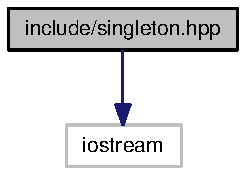
\includegraphics[width=77pt]{singleton_8hpp__incl}
\end{center}
\end{figure}
\subsection*{Classes}
\begin{CompactItemize}
\item 
class \hyperlink{classSingleton}{Singleton$<$ T $>$}
\begin{CompactList}\small\item\em Template de classe permettant de rendre une classe instanciable une seule fois. \item\end{CompactList}\end{CompactItemize}


\subsection{Detailed Description}
Implementation du design pattern singleton. 

\begin{Desc}
\item[Author:]GDD 

Arnaud Faure 

Pauline Requena \end{Desc}
\begin{Desc}
\item[Version:]0.1 \end{Desc}
\begin{Desc}
\item[Date:]29 mars 2009\end{Desc}
Implementation du design pattern singleton pour rendre une classe instanciable une unique fois. 
\printindex
\end{document}
